The scenario $\xi=(\E,\C)$ is in \emph{normalised form} iff
every event of \E{} has only one occurrence in \E{}\footnote{
%An arbitrary scenario can be trivially transformed to normalized
%form.
If there is more than one event with the same name, say $a$, in a scenario
of length $n$, the $k$th ($1<k\leq n-1$) occurrence of
$a$ can be replaced with $a_{k}$.}.
%In the rest of the paper we assume all the sequential scenarios are
%normalized.
If $\xi$ is in normalised form, then each event is uniquely
identified by its name.
If event $i$ in $\xi$ is $a$, we will use $t_a$
(instead of $t_i$) to refer to the time of $a$ in a behaviour
$\Behaviour{B}\in \Sem{\xi}$. If event $j$ ($i<j$) in
$\xi$ is $b$, we will use $\TT{a}{b}$ (instead of \TT{i}{j}) in a
constraint that restricts the time distance between $a$ and $b$, and
$\T{a}{b}^\Behaviour{B}$ (instead of $\T{i}{j}^\Behaviour{B}$) to
represent the time distance between $a$ and $b$ in \Behaviour{B}.
%For a consistent and normalised scenario $\xi = (\E, \C)$ over
%$\Sigma$, where $\E = e_0 e_1 \dots e_n$, we use
%$\Sigma_{\xi}= \{e_0, e_1, \dots, e_n \} \subseteq \Sigma$ to denote
%the set of events in $\E$.
%We assume $\Sigma_{\xi}$ includes the event \Dash.
%We explain the motivation for this after \Def{def-sync-event}.
Naturally, the sequence $\E = e_o e_1 ... e_{n}$ of a normalised scenario $\xi$ induces a
total order on $\Sigma_{\xi}$. We use $\TotalS{\xi}$ to denote this
total order: for two events $e_i$ and $e_j$ in
$\E$, $e_i \TotalS{\xi} e_j \iff i < j$.

A \emph{distributed timed scenario} (\emph{DTS} or \emph{distributed
scenario} for short) over $\Sigma$ is a finite collection of
(sequential) scenarios, denoted by $\DScenario=\D(\xi_1,\dots,\xi_n)$,
such that each $\xi_j$ ($1\leq j \leq n$) is consistent and is in
normalised form.
We refer to each $\xi_j$ as a \emph{component of} \DScenario.
  We use $\Sigma_{\DScenario} = \Sigma_{\xi_1} \cup \dots \cup
  \Sigma_{\xi_n}\subseteq\Sigma$ to denote the set of events of \DScenario.
  We say \DScenario{} % over $\Sigma$ is
is \emph{well-formed} iff $\ParS{\DScenario}\subseteq \Sigma_{\DScenario} \times
\Sigma_{\DScenario}$, defined as the transitive closure of $\bigcup_{\xi \in \Xi}
\TotalS{\xi}$, is a strict partial order on $\Sigma_{\DScenario}$.

For $\Behaviour{B}$, a behaviour over $\Sigma$, and $\xi$, a
scenario, such that $\Sigma_{\xi} \subseteq \Sigma$,
the \emph{restriction} of \Behaviour{B} to $\xi$, denoted by
$\Behaviour{B}_{\xi}$, is the maximal subsequence of \Behaviour{B} such that
every event of $\Behaviour{B}_{\xi}$ is in $\Sigma_{\xi}$.
If $\DScenario=\D(\xi_1,\dots,\xi_n)$ is a DTS
over $\Sigma$, then behaviour \Behaviour{B} over
$\Sigma$ is
\emph{allowed} by \DScenario{} iff, for every component $\xi_i$ of \DScenario{}
($1\leq i\leq n$), $\Behaviour{B}_{\xi_i} \in \Sem{\xi_i}$.
Clearly, if \DScenario{} is not well-formed, then it allows no behaviours.
The \emph{semantics} of \DScenario,
denoted by \Sem{\DScenario}, is the set of behaviours that are allowed
by \DScenario.
A DTS \DScenario{} is \emph{consistent}
iff $\Sem{\DScenario} \neq \emptyset$.
%It is \emph{inconsistent} iff $\Sem{\DScenario}=\emptyset$.
% NEDA: IF WE NEED EQUIVALENCE< RESTORE.
%Two consistent distributed scenarios, $\DScenario$ and $\DScenario'$,
%over $\Sigma$, are \emph{equivalent} (denoted by $\DScenario \equiv
%\DScenario'$) iff $\Sem{\DScenario} = \Sem{\DScenario'}$.
For a DTS \DScenario{}, and $e \in \Sigma_\DScenario{}$ if
  $|\Set{\xi \in \DScenario}{e \in \Sigma_{\xi}}| > 1$, then $e$ is
  called a \emph{synchronising event} for \DScenario{}\footnote{
  %Since the components of a DTS are in normalised form,
  We assume that any renaming of the synchronising events necessitated by normalising
  the components of a DTS is performed consistently
  across all the components. This does not pose any practical limitations.}.
  %If an event, say $a$, has more than one occurrence in a component of a DTS,
  %and $a$ is a synchronising event, then

For example, $\DScenario_1 = \D(\xi_1,\xi_2)$, where
 $\xi_1 = (habc, \{\TT{h}{a} \leq 3, \TT{a}{b} \leq
 4\})$ and $\xi_2 =
 (hefbd, \{\TT{h}{e} \geq 4\})$ is a consistent DTS:
 behaviour $\Behaviour{B} = (h,0)
 (a,3)(e,5)(f,6)(b,7)$\\$(c,9)(d,10)$ is in $\Sem{\DScenario_1}$.
 This is because $\Behaviour{B}_{\xi_1} = (h, 0) (a, 3)(b,
 7)(c, 9)$ is in $\Sem{\xi_1}$
and $\Behaviour{B}_{\xi_2} =  (h, 0) (e, 5)(f, 6)(b, 7)(d,10)$ is in
$\Sem{\xi_2}$.
Notice that $\Behaviour{B}$ consists of an
interleaving of the timed events of $\xi_1$ and $\xi_2$, except that
the events \emph{h} and \emph{b} occur only once. These events,
which occur simultaneously in $\xi_1$ and $\xi_2$, are the
synchronising events of $\DScenario_1$.
One can think of the behaviours of the components of $\DScenario_1$ as
taking place concurrently, but synchronising on the shared events
(``rendezvous'' synchronisation).
In other words, $\DScenario_1$ can be viewed as a \emph{parallel composition} of
its components.
If $\DScenario=\D(\xi_1,\dots,\xi_n)$, then we often write
$\DScenario=\xi_1\Vert\dots\Vert\xi_n$.

{\bf Distance relations} If $\DScenario=\D(\xi_1,\dots,\xi_n)$, where
$\xi_i=(\E_i,\C_i)$ ($1\leq i \leq n$), then let
$\C(\DScenario)=\bigcup_{1\leq i \leq n}\C_i$.
  If \DScenario{} is a well-formed DTS, for
  $(e_1,e_2) \in \PR{\DScenario}$, we define
$L_{e_1e_2} = \Set{l}{\TT{e_1}{e_2}\geq l \in \C(\DScenario)}$
and
$H_{e_1e_2} = \Set{h}{\TT{e_1}{e_2}\leq h \in \C(\DScenario)}$.
The distance relation of \DScenario{}
%\DR{\DScenario}, is the pair
is $\DR{\DScenario}=(\PR{\DScenario},\DF{\DScenario})$,
where
 $\DF{\DScenario}: \PR{\DScenario} \mapsto  \mathbb{Q}\times  \mathbb{Q}$ is a
  total function and
$\DF{\DScenario}(e_1,e_2)=[l_{e_1e_2},h_{e_1e_2}]$, such that
(i) if $L_{e_1e_2} \neq \emptyset$, then
%$l_{e_1e_2}= \max\{l~|~l \in L_{e_1e_2}\}$,
$l_{e_1e_2}= \max(L_{e_1e_2})$,
otherwise $l_{e_1e_2}=0$ and
(ii) if $H_{e_1e_2} \neq \emptyset$, then
%$h_{e_1e_2}= \min\{h~|~h \in H_{e_1e_2}\}$,
$h_{e_1e_2}= \min(H_{e_1e_2})$,
otherwise $h_{e_1e_2}=\infty$.
    $\DR{\DScenario}$ is
   \emph{stable} iff for every $e_1\PR{\DScenario} e_2$, $l_{e_1e_2} \leq
   h_{e_1e_2}$, and for every $e_1\PR{\DScenario} e_2\PR{\DScenario}e_3$, the
   following inequalities hold
\setlength\abovedisplayskip{2pt}
\setlength\belowdisplayskip{2pt}
\begin{equation}
  \label{golden2}
  %\begin{math}
  \Low{e_1}{e_2}+ \Low{e_2}{e_3} \leq \Low{e_1}{e_3} \leq
  \left\{
  \begin{array}{l}
    \Low{e_1}{e_2}+ \High{e_2}{e_3}\\
    \High{e_1}{e_2}+ \Low{e_2}{e_3}
  \end{array}
  \right \}
  %\end{math}
  \leq \High{e_1}{e_3} \leq \High{e_1}{e_2}+ \Low{e_2}{e_3}
\end{equation}
\noindent
If \DScenario{} is consistent, $\DR{\DScenario}$ can be
stabilised by iteratively applying the rules shown in \Fig{fig-rules}.
We use $\DRS{\DScenario}=(\PR{\DScenario},\DFS{\DScenario})$ to denote
the stable distance relation of \DScenario{}.
\DFS{\DScenario} maps $(e,e')$ in
$\PR{\DScenario}$ to an interval
%, interpreted as a pair of constraints
%(which might be \emph{implied} \cite{neda2020-2} by
%the original intervals in \DFS{\DScenario}),
which corresponds to the
%that specify the
lower and upper bounds on the time distance between $e$ and
$e'$ in all the behaviours of \DScenario.
%-------------------------------------
\begin{figure}[t]
\begin{center}
   \adjustbox{valign=b}
        {\begin{minipage}{0.62\linewidth}
   %      \tikz \node [scale=0.98] {
        %  \begin{center}
 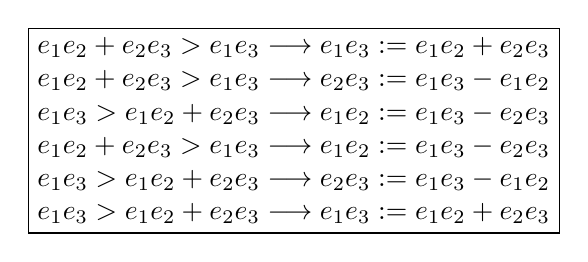
\begin{tikzpicture}[every text node part/.style={align=left}]
        \node (n1) at (0,0) [rectangle, draw]
        {
%        \begin{gather*}
 $\Low{e_1}{e_2} + \Low{e_2}{e_3} > \Low{e_1}{e_3}
  \longrightarrow \Low{e_1}{e_3} := \Low{e_1}{e_2} + \Low{e_2}{e_3}$\\

   $\Low{e_1}{e_2} + \High{e_2}{e_3} > \High{e_1}{e_3}
 \longrightarrow \High{e_2}{e_3} := \High{e_1}{e_3} - \Low{e_1}{e_2}$\\

  $\Low{e_1}{e_3} > \Low{e_1}{e_2} + \High{e_2}{e_3}
  \longrightarrow \Low{e_1}{e_2} := \Low{e_1}{e_3} - \High{e_2}{e_3}$\\

 $\High{e_1}{e_2} + \Low{e_2}{e_3} > \High{e_1}{e_3}
 \longrightarrow \High{e_1}{e_2} := \High{e_1}{e_3} - \Low{e_2}{e_3}$\\

$\Low{e_1}{e_3} > \High{e_1}{e_2} + \Low{e_2}{e_3}
  \longrightarrow \Low{e_2}{e_3} := \Low{e_1}{e_3} - \High{e_1}{e_2}$\\

 $\High{e_1}{e_3} > \High{e_1}{e_2} + \High{e_2}{e_3}
 \longrightarrow \High{e_1}{e_3} := \High{e_1}{e_2} + \High{e_2}{e_3}$
%\end{gather*}
               };
            %  \node (n1) at (0,-1.1) [rectangle, draw = none]{$\gamma$};
      \end{tikzpicture}
      %  \end{center}
 %       };
      \caption{Rules for stabilising a distance relation}
\label{fig-rules}
\vspace{-5mm}
    \end{minipage}}
\adjustbox{valign=b}
 {\begin{minipage}{0.37\linewidth}
\adjustbox{valign=b}
 {\begin{minipage}{0.49\linewidth}
 \begin{center}
 %               \adjustbox{valign=b}
%{\begin{minipage}{0.49\linewidth}
  \begin{tikzpicture}
    \tikzset{vertex/.style = {shape=circle,draw,minimum size=1em}}
    \tikzset{vertex3/.style = {shape=circle,draw,minimum size=1.5em}}
    \tikzset{vertex2/.style = {shape=rectangle,draw=none,minimum size=0.5em}}
    \tikzset{edge/.style = {-,> = latex'}}

    % vertices

    \node[vertex2] (b) at  (0,-0.7) {$h$};

    \node[vertex2] (x) at  (0,-1.4) {$a$};
\node[vertex2] (y) at  (1,-1.1) {$e$};
\node[vertex2] (z) at  (1,-1.8) {$f$};
    \node[vertex2] (e) at  (0,-2.1) {$b$};

    \node[vertex2] (f) at  (0,-2.8) {$c$};
   \node[vertex2] (g) at  (1,-2.5) {$d$};
       %edges
  %  \draw[edge] (b) to node[right ]{$[0]$} node[left]{$a$} (x);
 \draw[edge] (b) to (x);
    \draw[edge] (x) to (e);
    \draw[edge] (e) to (f);
   %  \draw[edge] (e) to (g);
      \draw[edge] (b) to (y);
       \draw[edge] (y) to (z);
        \draw[edge] (z) to (e);
        \draw[edge] (e) to (g);
    \end{tikzpicture}
 %    \caption{$\PR{\DScenario}$}
   %  maximal chains ($\DScenario_1$)}
%     \label{fig-chains}
     \end{center}
    \end{minipage}}
    \adjustbox{valign=b}
     {\begin{minipage}{0.49\linewidth}
 \begin{center}
 %               \adjustbox{valign=b}
%{\begin{minipage}{0.49\linewidth}
  \begin{tikzpicture}
    \tikzset{vertex/.style = {shape=circle,draw,minimum size=1em}}
    \tikzset{vertex3/.style = {shape=circle,draw,minimum size=1.5em}}
    \tikzset{vertex2/.style = {shape=rectangle,draw=none,minimum size=0.5em}}
    \tikzset{edge/.style = {-,> = latex'}}

    % vertices

    \node[vertex2] (b) at  (0,-0.3) {$h$};

    \node[vertex2] (x) at  (0,-0.9) {$a$};
\node[vertex2] (y) at  (1,-1.2) {$e$};
\node[vertex2] (z) at  (1,-1.8) {$f$};
    \node[vertex2] (e) at  (0,-2) {$b$};
    \node[vertex2] (f) at  (0,-2.6) {$c$};
   \node[vertex2] (g) at  (1,-2.5) {$d$};
       %edges
  %  \draw[edge] (b) to node[right ]{$[0]$} node[left]{$a$} (x);
 \draw[edge] (b) to (x);
    \draw[edge] (x) to (e);
    \draw[edge] (e) to (f);
     \draw[edge] (x) to (y);
      \draw[edge] (b) to (y);
       \draw[edge] (y) to (z);
        \draw[edge] (z) to (e);
        \draw[edge] (e) to (g);
    \end{tikzpicture}
 %    \caption{$\PR{\DScenario}$}
   %  maximal chains ($\DScenario_1$)}
 %    \label{fig-chains}
     \end{center}
    \end{minipage}}
 \caption{$\PR{\DScenario_1}$ and $\ParSE{\DScenario_1}$}
   %  maximal chains ($\DScenario_1$)}
     \label{fig-chains}
     \vspace{-5mm}
 \end{minipage}}
   \end{center}
  \end{figure}
%-----------------------


We represent a partial order by its maximal chains, visually
represented by a Hasse diagram. For $\DScenario_1$,
$\PR{\DScenario_1}$ is shown in \Fig{fig-chains},
%The stable distance function of $\DScenario_1$,
$\DFS{\DScenario_1}$ is represented by
$\{(h, a, 0, 3),
(h, b, 4, 7),
(h, c, 4, \infty),
(h, d, 4, \infty),
(h, e, 4, 7),
(h, f, 4, 7),
(a, b, 1, 4),\\
(a, c, 1, \infty),
(a, d, 1, \infty),
(e, b, 0, 3),
(e, f, 0, 3),
(f, b, 0, 3)\}$.
Tuples of the form\\ $(e,e',0,\infty)$ (indicating default
constraints) will not be included in our examples.
%----------------------------

{\bf Extended distance relations}
The \emph{extended partial order} of $\DScenario$,
$\ParSE{\DScenario}: \Sigma_{\DScenario} \times  \Sigma_{\DScenario}$,
is the smallest relation
that satisfies the following conditions: (i) if
$e\PR{\DScenario}e'$, then $e\ParSE{\DScenario}e'$; (ii) if there
exists $o\in\Sigma_{\DScenario}$ such that $o\ParSE{\DScenario}e$,
$o\ParSE{\DScenario}e'$ and $\Max{o}{e} < \Min{o}{e'}$
 in $\DFS{\DScenario}$,
or $e\ParSE{\DScenario}o$, $e'\ParSE{\DScenario}o$ and $\Max{e'}{o}
< \Min{e}{o}$ in $\DFS{\DScenario}$, then $e\ParSE{\DScenario}e'$;
(iii) if $e\ParSE{\DScenario}e'$ and  $e'\ParSE{\DScenario}e''$, then
$e\ParSE{\DScenario}e''$.
%the transitive closure of $\ParS{\DScenario}$
The \emph{initial} extended distance relation of \DScenario{} is
%  $\DRS{\DScenario}=(\PR{\DScenario},\DFS{\DScenario})$ is
 $\DRE{\DScenario}=(\ParSE{\DScenario},\DFEX{\DScenario})$,
where
    $\DFEX{\DScenario}(e, e') = [0,\infty]$ if
$(e,e')$ in $\ParSE{\DScenario}\setminus \ParS{\DScenario}$,
and $\DFEX{\DScenario}(e, e') = \DFS{\DScenario}(e, e')$ if
 $(e,e')$ in $\ParS{\DScenario}$.
The \emph{stable extended distance relation} of $\DScenario$,
denoted by $\DRSE{\DScenario}=(\ParSE{\DScenario},\DFE{\DScenario})$, is
obtained by stabilising $\DRE{\DScenario}$.

In $\DScenario_1$, $\Max{h}{a}=3 < \Min{h}{e}=4$ in $\DFS{\DScenario_1}$,
so $\PR{\DScenario_1}$ can be extended with $(a,e)$ (see
$\ParSE{\DScenario_1}$ in \Fig{fig-chains}) and
$\DFE{\DScenario_1}=\DFS{\DScenario_1}\cup\{(a,e,1,4),(a,f,1,4)\}$.

To avoid visual clutter
%in the rest of the text,
we will use
$\DR{\DScenario}=(\ParS{\DScenario},\DF{\DScenario})$ for the stable
extended distance relation of $\DScenario$.
A (sequential) scenario, $\xi$, can be seen as a trivial DTS,
$\D(\xi)$. We use $\DR{\xi}=(\ParS{\xi},\DF{\xi})$ for its stable
distance relation, where $\PR{\xi}$ is $\TotalS{\xi}$.

%\noindent
{\bf Realisability of (sequential) scenarios as distributed
scenarios}
Let $\mathcal{S}=\{\SeqS_1,\dots,\SeqS_n\}$, such that each
$\SeqS_i\in\mathcal{S}$ has a
different sequence of events, and
each event in $\Sigma_{\mathcal{S}}$ occurs exactly once in each $\SeqS_i$.
If there exists a DTS
$\DScenario$ over $\Sigma_{\mathcal{S}}$, such
that $\Sem{\DScenario} = \bigcup_{1\leq i \leq
n} \Sem{\SeqS_{i}}$, we say $\mathcal{S}$ is \emph{realisable} by
$\DScenario$.

%----------------------
{\bf Projections of distance relations}
Let $\DR{}=(\ParS{},\DF{})$ be a
stable distance relation over $\Sigma$.
A \emph{projection} of $\DR{}$ is a
scenario $\xi_p = (p, \C_p)$, where
(i) $p$ is a permutation of events in $\Sigma$ that
agrees with $\ParS{}$, and
(ii) $\C_{p}$ is a set of constraints:
for every $e$ and $e'$ such that $e$ appears before
$e'$ in $p$,
if $e\not\ParS{}e'$, then the default constraints
$0 \leq \TT{e}{e'}\leq \infty$ are added to $\C_p$,
otherwise the constraints
$l \leq \TT{e}{e'} \leq h$ are added to $\C_{p}$, where
$\DF{}(e,e')=[l,h]$.
When we create $\DR{\xi_p}$, we must, of course, stabilise it.
In the rest of the text we assume the distance relations of all
the projections are stabilised.

The set of all the projections obtained in this way is realisable by
any DTS for which $\DR{}$ is the extended distance relation.
Moreover, given the extended distance relation $\DR{}$ for a DTS
\DScenario, the set of projections of $\DR{}$ uniquely determines the
semantics of \DScenario: every behaviour in $\Sem{\DScenario}$ is allowed by
one projection.
%-------------------------------
